\documentclass[11pt]{article}
\usepackage[margin=20mm]{geometry}
\usepackage{amsmath}
\usepackage{listings,color,enumitem}
\definecolor{mygreen}{RGB}{28,172,0} % color values Red, Green, Blue
\definecolor{mylilas}{RGB}{170,55,241}
\usepackage{graphicx}
\title{Homework 1\\ \vspace{2mm}\Large{16-720A Computer Vision }}
\author{Matthew Swenson}

\begin{document}
	\maketitle
	
\section{Question 1.0}
    \begin{enumerate}
    \item The Gaussian filters detect local neighborhood features. 
    \item The Laplacian of Gaussian filters detect rapid changes in features (edges and corners in both directions). 
    \item The dx filters detect changes along the x axis of the image. 
    \item The dy filters detect changes along the y axis of the image. 
    \end{enumerate}
    All of the filters are scaled such that they detect progressively larger features. 
\begin{figure}[ht]
\centering
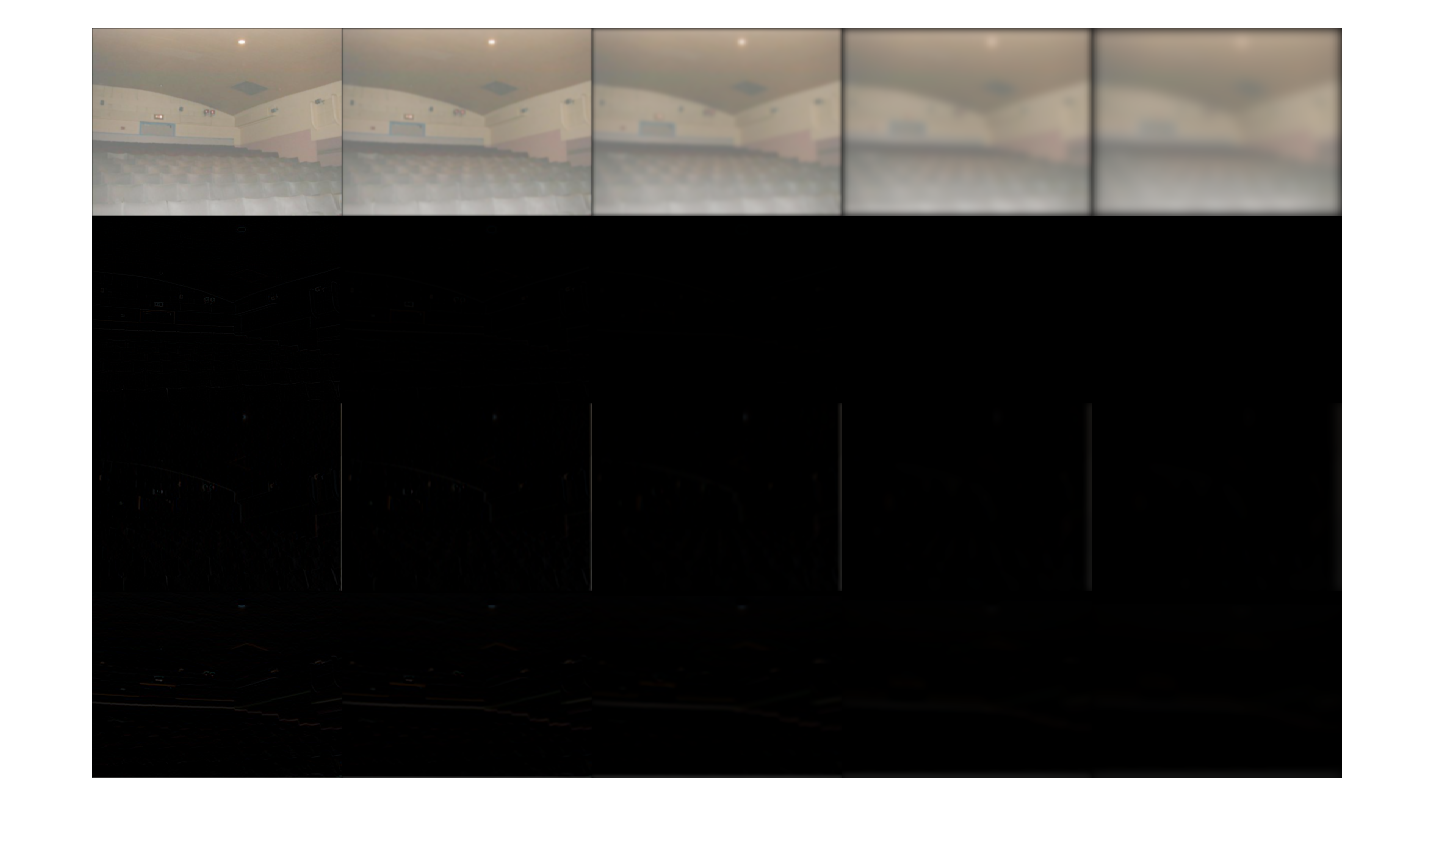
\includegraphics[width=1.0\textwidth]{filter_responses.png}
\caption{The various filter responses of a picture of an auditorium. Rows are Gaussian, LoG, dX, dY.
Columns are increasing scale of filter. }
\end{figure}
\section{Question 1.3}
Section 1.3 involved the creation of "wordmaps" of each image using the computed dicitonary;
namely matching the closest texton to each pixel of an image in an attempt to generalize image
textures. This was reasonably successful, as depicted in the assiociated image. I found it somewhat
surprising that areas that look extremely visually similar to me are often classified as different
textons; such as parts of the sky in the windmill picture, or even more confusingly, parts of the 
cabinents in the kitchen picture. 
\begin{figure}[ht]
\centering
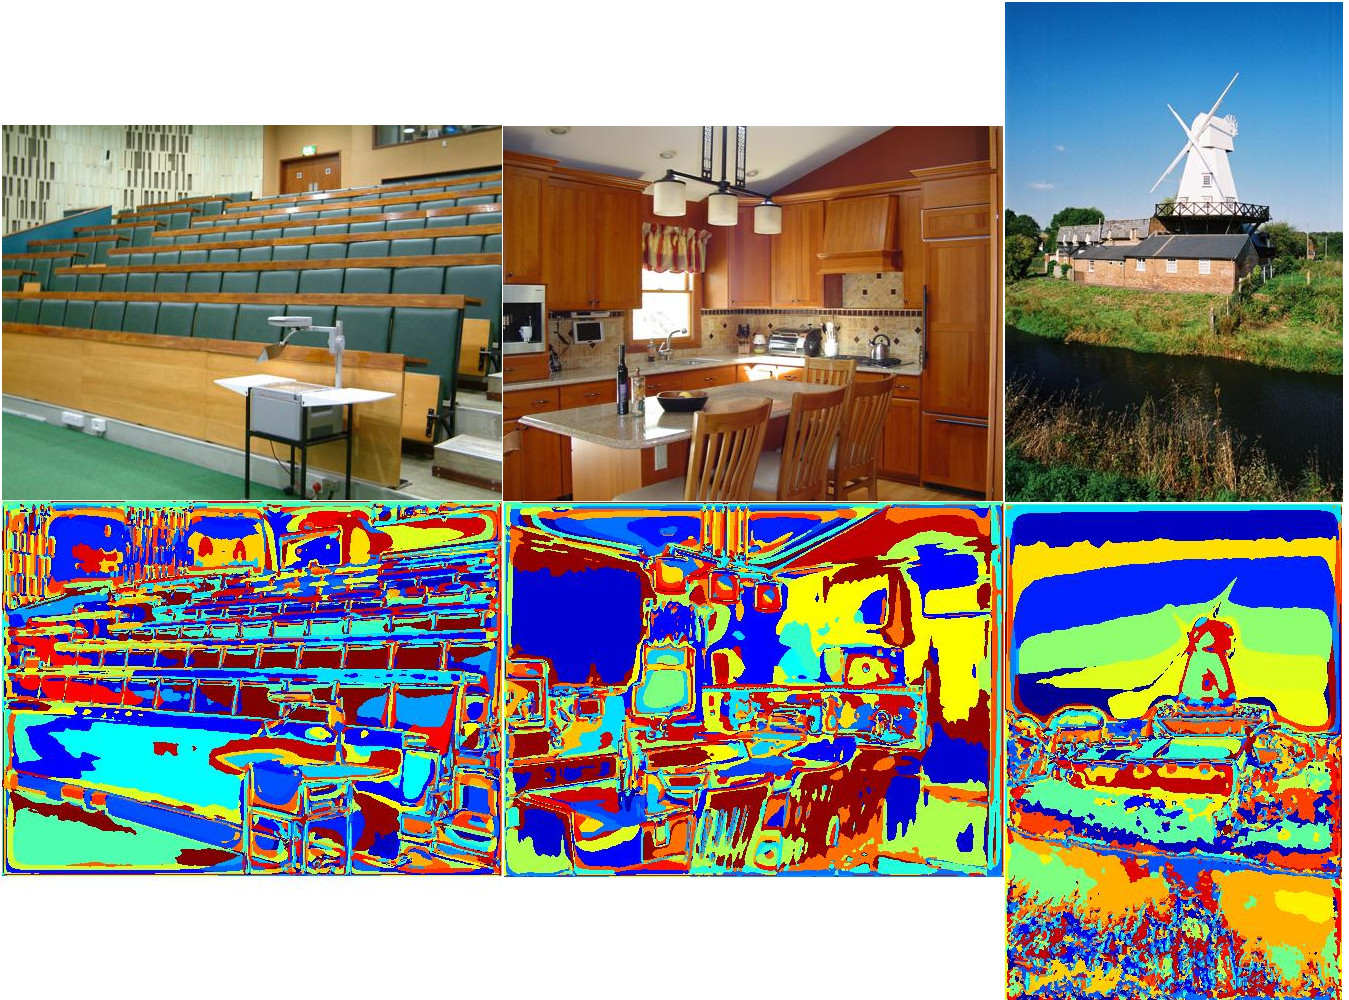
\includegraphics[width=\textwidth]{wordmaps.jpg}
\caption{Various false-color wordmaps of images. Each hue is the closest texton to that part of the real image. }
\end{figure}
\section{Question 2.5}
 The overall accuracy of this system is 56.25\%, for $\alpha$=400 and $K=175$. 
\begin{table}[h!]
\centering
\caption{Confusion Matrix }
\label{conf}
\begin{tabular}{|c|c|c|c|c|c|c|c|c|}\hline
&\textit{auditorium} & \textit{baseball field} & \textit{desert} & \textit{highway} & \textit{kitchen} & \textit{laundromat} & \textit{waterfall} & \textit{windmill} \\ \hline
\textit{auditorium}     & \textbf{12} &  2  &  0 &   0 &   4 &   1 &   1 &   0 \\ \hline
\textit{baseball field} & 0   &\textbf{11}  & 2  &  1  &  1  &  0  &  2  &  0  \\ \hline
\textit{desert}         & 0   & 3   & \textbf{9} &  3  &  0  &  0  &  0  &  0  \\ \hline
\textit{highway}        & 0   & 0   & 4  &\textbf{ 12} &  0  &  1  &  1  &  8  \\ \hline
\textit{kitchen}        & 3   & 1   & 2  &  0  & \textbf{13} &  9  &  0  &  0  \\ \hline
\textit{laundromat}     & 3   & 0   & 1  &  0  &  1  &  \textbf{9}  &  1  &  0  \\ \hline
\textit{waterfall}      & 1   & 0   & 0  &  1  &  1  &  0  &\textbf{14}  &  2  \\ \hline
\textit{windmill}       & 1   & 3   & 2  &  3  &  0  &  0  &  1  & \textbf{10} \\ \hline 
\end{tabular}
\end{table}
\section{Question 2.6}
The single greatest source of error in the system was the misclassification of kitchens as laundromats.
Intuitively, this makes sense, as both kitchens and laundromats feature a significant number of 
similar scale rectangular appliances, counters, and chairs, and often have similar layouts. 

Slightly more confusing is the high number of highways that were misclassified as windmills.
My guess is that both of these image sets feature lots of sky and grassy areas, with a darker
line shaped object running up the middle, and because the system primarily looks for textures,
a lot of those images are going to be very similar. 


\end{document}
